\section{Nearest particle statistics}

To circumvent this issue of diverging integral we introduce the \textit{Nearest neighbor statistic} in the form introduced \citet{zhang2021ensemble}. 
As the computation of the wake of the particle requires the knowledge of its velocity, we modify slightly the \textit{Nearest neighbor statistics} of \citet{zhang2021ensemble} to include a condition on the \textit{test } particle center of mass velocity.
Therefore, in the first place we introduce the \textit{Nearest neighbor velocity included} distribution as, 
\begin{equation}
    P_\text{nst}^f[\textbf{x},\textbf{r},\textbf{w},t]
    = \frac{1}{\phi_f}\avg{
        \chi_f[\textbf{x},t]
        \sum_i^N 
        \delta(\textbf{x}_i[\FF,t]-\textbf{y})
        \delta(\textbf{u}_i[\FF,t]-\textbf{w})
        h_i[\textbf{x},\FF,t]
    },
\end{equation}
where,
\begin{align}
    h_i[\textbf{x},\FF,t]
    = \frac{1}{N[\textbf{x},t,\FF]}
    \prod_j H(|\textbf{x}_j[\FF,t] - \textbf{x}| - |\textbf{x}_i[\FF,t] - \textbf{x}|)\\
    N[\textbf{x},t,\FF]
    = \sum_i\prod_jH(|\textbf{x}_j[\FF,t] - \textbf{x}| - |\textbf{x}_i[\FF,t] - \textbf{x}|).
\end{align}
It must be understood from this definition that $h_i=1$ if and only if the particle $i$ is the nearest neighbor to the point $\textbf{x}$. 
With that definition, $P_\text{nst}^f$ is the probability of finding the continuous the nearest neighbor of the point \textbf{x} located at \textbf{y} with a velocity \textbf{w} at time $t$, knowing that the continuous phase is present at \textbf{x}. 

By noticing that, 
\begin{equation}
    \int_{\mathcal{R}^6}
    \sum_i^N 
    \delta(\textbf{x}_i[\FF,t]-\textbf{y})
    \delta(\textbf{u}_i[\FF,t]-\textbf{w})
    h_i[\textbf{x},\FF,t]
    d\textbf{r}
    d\textbf{w} 
    =1,
\end{equation}
we arrive at the same conclusion as \citet{zhang2021ensemble} and write, 
\begin{equation}
    \avg{f_f^0\chi_f}
    = 
    \int_{\mathbb{R}^6}
    (f_f^\text{nst}P_\text{nst}^f\phi_f)[\textbf{x},\textbf{r},\textbf{w},t]
    d\textbf{r}
    d\textbf{w}
    \label{eq:ensemble_avg_to_nst}
\end{equation} 
where $f_f^0[\textbf{x},\FF,t]$ is an arbitrary property pertaining to the continuous phase, and $f_f^\text{nst}[\textbf{x},t|\textbf{w},\textbf{y}]$ is its conditional averaged on the presence of a nearest neighbor at \textbf{y} with velocity \textbf{w} and with the continuous phase at \textbf{x}, namely, 
\begin{equation}
    f_f^\text{nst}[\textbf{x},t|\textbf{w},\textbf{y}]
    =\frac{1}{(P_\text{nst}^f\phi_f) [\textbf{x},\textbf{r},\textbf{w},t]}
    \avg{
        (f_f^0
        \chi_f)[\textbf{x},t]
        \sum_i^N 
        \delta(\textbf{x}_i[\FF,t]-\textbf{y})
        \delta(\textbf{u}_i[\FF,t]-\textbf{w})
        h_i[\textbf{x},\FF,t]
    }.
    \label{eq:def_f_nst}
\end{equation}
Note that the only difference between these definitions and the definitions presented in \citet{zhang2021ensemble}, i.e. Equation (2.6) to (2.8) of \citet{zhang2021ensemble}, is the inclusion of $\delta(\textbf{u}_i - \textbf{w})$ in our formulas. 
Anyhow, \ref{eq:ensemble_avg_to_nst} permitted us to express any ensemble averaged quantities in terms of \textit{Nearest neighbor conditioned} quantities. 
Therefore, this formula is in fact a tool similar to \ref{eq:batchlor_avg} but derived without any assumption, meaning with absence of errors. 

In the following we introduce the shorthand, 
\begin{equation*}
    \delta_\text{nst}^f [\textbf{x},\textbf{y},\textbf{w},t,\FF]
    =
    % \chi_f
    \sum_i^N 
    \delta(\textbf{x}_i[\FF,t]-\textbf{y})
    \delta(\textbf{u}_i[\FF,t]-\textbf{w})
    h_i[\textbf{x},\FF,t],
\end{equation*}
so that the conditional nearest neighbor average can simply be written, $f_f^\text{nst} P_\text{nst}^f \phi_f = \avg{\chi_f f_f^0 \delta_\text{nst}}$.

\subsection{A new Reynolds stress formulation}

Now, let us apply \ref{eq:ensemble_avg_to_nst} to the quantity of interest, specifically $f_f^0 = \textbf{u}_f'\textbf{u}_f'$, which yields: 
\begin{equation}
    \avg{\chi_f \textbf{u}_f'\textbf{u}_f'}
    = 
    \phi_f
    \int_{\mathbb{R}^6}
    \textbf{v}_f^\text{nst}
    \textbf{v}_f^\text{nst}
    P_\text{nst}^f
    d\textbf{r}
    d\textbf{w}
    + 
    \int_{\mathbb{R}^6}
    \avg{
        \chi_f
        \textbf{v}_f''
        \textbf{v}_f''
        % \sum_i 
        % \delta(\textbf{x}+\textbf{r}-\textbf{x}_i)
        % \delta(\textbf{w}-\textbf{u}_i)
        % h_i
        \delta_\text{nst}
    }
    d\textbf{r}
    d\textbf{w}
    \label{eq:relation_ensemble_nst}
\end{equation}
where we have defined: 
The fluctuation of the local value of the fluid phase velocity around the single particle conditional average $\textbf{v}_f'' = \textbf{u}_f^0 - \textbf{u}_f^\text{nst}$, and the fluctuation of the single particle nearest neighbor conditional average, around the ensemble average velocity, that is $\textbf{v}_f^\text{nst} = \textbf{u}_f^\text{nst} - \textbf{u}_f$. 
According to this definition, 
we state that we can separate the \textit{Reynolds stress} tensor into two distinct contributions :  (1) the agitation generated due to the averaged nearest neighbor averaged wakes around the particles at \textbf{y}, and (2) all other source of fluctuations such as those generated through particles interactions and the single phase turbulence. 
Note that, this decomposition is similar than those used in \ref{eq:classic_avg} and \ref{eq:batchlor_avg}, the only difference is the presence of the \textit{nearest neighbor} averaged fields instead of the classic single-particle conditioned averaged fields. 

To give a better physical explanation of what is $\textbf{u}_f^\text{nst}$ we display on \ref{fig:unst} an instantaneous representation of the meaning of $\textbf{u}_f^\text{nst}$. 
\begin{figure}[h!]
    \centering
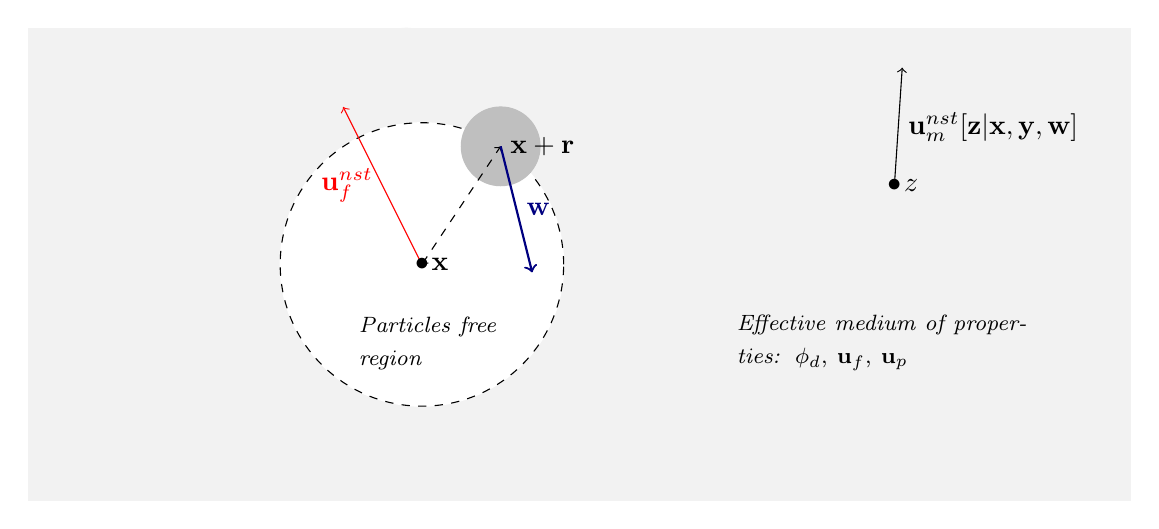
\begin{tikzpicture}
    \filldraw[gray!10](-5,-3) rectangle(9,3);
    \filldraw[white](0,0) circle (1.8);
    \filldraw[ gray!10!white](+2.6,0.5)circle (0.5);
    \filldraw[ gray!10!white](-1.5,2.2)circle (0.5);
    \draw[dashed](0:1.8) arc (0:360:1.8);
    % \filldraw[ gray!50!white](0,0) circle (0.5);
    \filldraw[ gray!50!white](1,1.5)circle (0.5);
    \filldraw[ gray!10!white](-0.2,2.5)circle (0.5);
    \draw[->,red](0,0)--++(-1,2)node[midway,left]{$\textbf{u}_f^\text{nst}$};
    \draw(0,0)node{$\bullet$}node[right]{$\textbf{x}$};
    \draw[dashed,<->](0,0)--(1,1.5)node[right]{$\textbf{x}+\textbf{r}$};
    \draw[->,blue!50!black,thick](1,1.5)--++(0.4,-1.6)node[midway,right]{$\textbf{w}$};
    % \draw[dashed](-0.2,3.5);
    \node[text width=2cm] (title) at (0.2,-1) {\footnotesize\textit{Particles free region}};
    % \node[ultra thick] (title) at (-0.5,-1.5) {(\textit{Case 1})};
    \node[text width=4cm] (title) at (6,-1) {\footnotesize\textit{Effective medium of properties:} $\phi_d$, $\textbf{u}_f$, $\textbf{u}_p$};
    \draw[->] (6,1)node{$\bullet$}node[right]{$z$}--++(0.1,1.5)node[right,midway]{$\textbf{u}_m^\text{nst}[\textbf{z}|\textbf{x},\textbf{y},\textbf{w}]$};
\end{tikzpicture} 
\caption{Representation of the \textit{nearest neighbor conditionally averaged} velocity fields $\textbf{u}_\text{nst}^f[\textbf{x},\textbf{w},\textbf{r},t]$, Inspired from (Figure 2) of \citet{zhang2021ensemble}}
\label{fig:unst}
\end{figure}
According to \ref{eq:def_f_nst} and \ref{fig:unst} $\textbf{u}_f^\text{nst}[\textbf{x},\textbf{r},\textbf{w}]$ is the averaged value of $\textbf{u}_f^0$, evaluated at \textbf{x}, on all configuration where a particle is present at $\textbf{y} = \textbf{x} + \textbf{r}$ with velocity $\textbf{w}$. 
Consequently, the region delimited by the sphere, centered at \textbf{x} of radius $|\textbf{y} - \textbf{x}|$ must be empty of particles center of mass \citep{zhang2021ensemble}. 
This deeper physical understanding will prove valuable in the subsequent section.  



\subsection{How to obtain the nearest neighbor conditional velocity fields ?}

In the objective of computing the sedimentation velocity, \citet[Appendix B]{zhang2021ensemble} has computed $\textbf{u}_f^\text{nst}$ using the \textit{nearest neighbor conditional averaged} Navier-Stokes equations. 
As his derivation does not provide detailed proof, especially on the derivation of Equation (B 1) of \citet{zhang2021ensemble},  we aim in this section to present a broader methodology. 

Inspired by the classic conditional average method of \citet{hinch1977averaged}, we stipulate that the nearest neighbor conditional velocity fields, i.e. $\textbf{v}_f^\text{nst}$,can be obtained by conditionally averaging the local scale mass and momentum equations, and solve for $\textbf{v}_f^\text{nst}$. 
Thus, let us first recall the local mass and momentum equation, 
\begin{align}
    \pddt (\rho_f\chi_f) +  \pddx \cdot (\rho_f\chi_f\textbf{u}^0_f) &= 0 \\
    \pddt (\rho_f\chi_f\textbf{u}^0_f)
    + \pddx\cdot (\rho_f\chi_f\textbf{u}^0_f\textbf{u}^0_f - \chi_f\bm\sigma^0_f)
    &= 
    - \delta_\Gamma \bm\sigma_f^0 \cdot \textbf{n}_d. 
    + \chi_f \rho_f \textbf{g}
    \label{eq:local_equations}
\end{align}
Then, note that we can obtain $\textbf{v}_f^\text{nst}$ from $\textbf{u}_f^0$ directly by the operation, 
\begin{equation*}
    \textbf{v}_f^\text{nst} P_\text{nst}^f
    = 
    \textbf{u}_f^\text{nst} P_\text{nst}^f
    - \textbf{u}_f P_\text{nst}^f
    = 
    \avg{\delta_\text{nst}^f \chi_f \textbf{u}_f^0}
    - \textbf{u}_f P_\text{nst}^f
\end{equation*}
We deduce that to obtain an equation for $\textbf{u}_f^\text{nst}$ we must multiply, \ref{eq:local_equations} by $\delta_\text{nst}$ and average overall configurations. 
This introduces the need of proper conservation equation for $\delta_\text{nst}$. 

\subsubsection{Conditionally mass transport equation}
Consequently, we introduce the  conservation equation of each distribution present in $\delta_\text{nst}$, it reads, 
\begin{align}
    \label{eq:dt_delta_x}
    \pddt \delta(\textbf{x}_i  - \textbf{y})
    +\textbf{u}_i  
    \cdot \pddy \delta(\textbf{x}_i  - \textbf{y})
    = 0\\
    \pddt \delta(\textbf{u}_i -\textbf{w})
    +\textbf{a}_i \cdot  \pddw   \delta(\textbf{u}_i  - \textbf{w})
    = 0\\
    \pddt \chi_f 
    + \textbf{u}_\Gamma^0 
    \cdot \pddx \chi_f = 0 \\
    \pddx \chi_f = - \delta_\Gamma \textbf{n}_f,
    \label{eq:chi_f_dt}
\end{align}
where we recall that $\textbf{u}_\Gamma^0$ is the velocity of the droplets interfaces, and $\textbf{n}_f$ is the normal pointing inward the droplets surfaces. 
Additionally, The vector $\textbf{a}_i$ correspond to the center of mass acceleration of the particle $i$. 
Form \ref{eq:dt_delta_x} to \ref{eq:chi_f_dt} we deduce that, 
\begin{align}
    \pddt \delta_\text{nst}
    + \pddy \cdot (\textbf{w} \delta_\text{nst})
    + \pddw \cdot (\textbf{a}_i  \delta_\text{nst})
    = 
    \sum_i \delta(\textbf{x}_i -\textbf{y}) \delta(\textbf{u}_i - \textbf{w}) \pddt h_i
\end{align}
% and, 
% \begin{align*}
%     \pddt (\chi_f \delta_\text{nst})
%     + \pddy \cdot (\textbf{w} \chi_f \delta_\text{nst})
%     + \pddw \cdot (\textbf{a}_i  \chi_f \delta_\text{nst})
%     = 
%     \chi_f \delta(\textbf{x}_i -\textbf{y}) \delta(\textbf{u}_i - \textbf{w}) \pddt h_i
%     + \delta_\Gamma \delta_\text{nst} \textbf{u}_\Gamma\cdot \textbf{n}_f
% \end{align*}
As, shown in appendix, 
\begin{align}
    \pddt  h_i[\textbf{x},t,\FF]
    = 
    h_i
    \sum_k 
    \delta(r_k - r_i)
    (\textbf{u}_k  \cdot \hat{\textbf{r}}_k - \textbf{u}_i  \cdot \hat{\textbf{r}}_i)\\
    \pddx  h_i[\textbf{x},t,\FF]
    = 
    h_i
    \sum_k 
    \delta(r_k - r_i)
    ( \hat{\textbf{r}}_k -  \hat{\textbf{r}}_i),
\end{align}
where we recall that $\textbf{u}_k$ and $\textbf{u}_i$  are the center of mass velocity of the particle $k$ and $i$ respectively.
Note that the second expression is in agreement with \citet[Appendix A]{zhang2021ensemble}. 
We also introduced the radial distance from the particle $i$ to the point $\textbf{x}$ namely, $r_i = |\textbf{x}_i - \textbf{x}|$.  
Anyhow, considering this relation yields a new expression for the transport equation of $\delta_\text{nst}$ namely,
\begin{equation}
    \pddt \delta_\text{nst}
    + \pddy \cdot (\textbf{w} \delta_\text{nst})
    + \pddw \cdot (\textbf{a}_i  \delta_\text{nst})
    = 
    % \sum_i
    % \delta(\textbf{x}_i -\textbf{y}) 
    % \delta(\textbf{u}_i - \textbf{w}) 
    \delta_\text{nst}
    % h_i
    \sum_k 
    \delta(r_k - r_i)
    (\textbf{u}_k  \cdot \hat{\textbf{r}}_k - \textbf{u}_i  \cdot \hat{\textbf{r}}_i). 
    % \label{eq:dt_delta_nst}
\end{equation}
As demonstrated in \citet{zhang2023evolution}, in another context, the right-hand side term of \ref{eq:dt_delta_nst} can be considered as a source term due to the birth or death of nearest neighbor to the point \textbf{x}. 
For reason that will become clear latter on we add the term $\textbf{u}_f^0\cdot \pddx \delta_\text{nst}$ on each side of the equation, which gives,
\begin{equation}
    \pddt \delta_\text{nst}
    + \textbf{u}_f^0\cdot \pddx \delta_\text{nst}
    + \textbf{w}   \cdot \pddy \delta_\text{nst}
    + \textbf{a}_i \cdot \pddw   \delta_\text{nst}
    = 
    % \sum_i
    % \delta(\textbf{x}_i -\textbf{y}) 
    % \delta(\textbf{u}_i - \textbf{w}) 
    \delta_\text{nst}
    % h_i
    \sum_k 
    \delta(r_k - r_i)
    ((\textbf{u}_k - \textbf{u}_f^0) \cdot \hat{\textbf{r}}_k - (\textbf{u}_i  - \textbf{u}_f^0)\cdot \hat{\textbf{r}}_i). 
    \label{eq:dt_delta_nst}
\end{equation}
On the right-hand side we have reformulated the term $\textbf{u}_f^0\cdot \pddx \delta_\text{nst}$, see \tb{Annexe} for the full derivation. 

To derive an equation for $P_\text{nst}^f$ we multiply \ref{eq:dt_delta_nst} by $\chi_f$, and make use of \ref{eq:chi_f_dt}, yielding, 
\begin{multline}
    \pddt (\chi_f\delta_\text{nst})
    +  \pddx \cdot (\textbf{u}_f^0 \chi_f\delta_\text{nst})
    +  \pddy \cdot (\textbf{w}    \chi_f\delta_\text{nst})
    +  \pddw \cdot   (\textbf{a}_i  \chi_f\delta_\text{nst})\\
    = 
    % \sum_i
    % \delta(\textbf{x}_i -\textbf{y}) 
    % \delta(\textbf{u}_i - \textbf{w}) 
    (\chi_f\delta_\text{nst})
    % h_i
    \sum_k 
    \delta(r_k - r_i)
    ((\textbf{u}_k - \textbf{u}_f^0) \cdot \hat{\textbf{r}}_k - (\textbf{u}_i  - \textbf{u}_f^0)\cdot \hat{\textbf{r}}_i). 
    \label{eq:dt_delta_nst_f}
\end{multline}
which upon averaging gives directly,
\begin{multline}
    \pddt (\phi_fP_\text{nst}^f)
    + 
    \pddx \cdot (
        \phi_f 
        P_\text{nst}^f
        \textbf{u}_f^\text{nst}
    )
    + \pddy \cdot (
        \phi_f
        P_\text{nst}^f
        \textbf{w} 
    )
    +
    \pddw \cdot (  
        \phi_f 
        P_\text{nst}^f
        \textbf{a}_p^\text{nst} 
    )
    = \\
    + \avg{
    %  \chi_f \textbf{u}_\Gamma \cdot \pddx \delta_\text{nst}
     \chi_f \delta_\text{nst}
    \sum_k 
    \delta(r_k - r_i)
    [(\textbf{u}_k - \textbf{u}_\Gamma^0) \cdot \hat{\textbf{r}}_k - (\textbf{u}_i- \textbf{u}_\Gamma^0)  \cdot \hat{\textbf{r}}_i]}.
    \label{eq:dt_P_nst_chi}
\end{multline}
where we have noted that $\textbf{u}_\Gamma^0 = \textbf{u}_f^0$ in the absence of mass transfer. 
In this relation the left-hand side terms represent the advection of $\phi_f P_\text{nst}^f$.
The source term on the right-hand side of \ref{eq:dt_delta_nst_chi} accounts for the changes in nearest neighbor distribution due to the permutation of the nearest neighbor at the local scale. 
Note the similarities of the right-hand side source term of \ref{eq:dt_delta_nst_chi} with (A10) of \citet{zhang2023evolution}, which derived a transport equation for $P_\text{nst}$ such as it is defined in the previous chapters. 
We remark that the source terms of (A10) and \ref{eq:dt_delta_nst_chi} yield the same form, but in \ref{eq:dt_delta_nst_chi} the velocity $\textbf{u}_i$ and $\textbf{u}_k$ are evaluated with respect to the local velocity of the fluid $\textbf{u}_f^0$, while in \citet{zhang2023evolution} it is evaluated relative to the velocity of the particles centered at \textbf{x}. 
This is not surprising considering the difference in definition between $P_\text{nst}^f$ and $P_\text{nst}$ in \citet{zhang2023evolution}. 


\ref{eq:dt_P_nst_chi} which can also be written in ``conservative'' form using \ref{eq:dt_P_nst_chi} and, 
\begin{equation}
    \pddt \phi_f 
    + \div(
        \phi_f
        \textbf{u}_f 
        ) 
    = 0, 
\end{equation}
to show that \ref{eq:dt_delta_nst_chi} can be written in ``conservative'' form, yielding, 
\begin{multline}
    \pddt P_\text{nst}^f
    + 
    \pddx \cdot (
        P_\text{nst}^f
        \textbf{u}_f^\text{nst}
    )
    + \pddy \cdot (
        P_\text{nst}^f
        \textbf{w}
    )
    +
    \pddw \cdot (  
        P_\text{nst}^f
        \textbf{a}_p^\text{nst} 
    )
    = \\
    + \frac{1}{\phi_f}\avg{
    %  \chi_f \textbf{u}_\Gamma \cdot \pddx \delta_\text{nst}
     \chi_f \delta_\text{nst}
    \sum_k 
    \delta(r_k - r_i)
    [(\textbf{u}_k - \textbf{u}_\Gamma^0) \cdot \hat{\textbf{r}}_k - (\textbf{u}_i- \textbf{u}_\Gamma^0)  \cdot \hat{\textbf{r}}_i]}.
    \label{eq:dt_Pc_nst_chi}
\end{multline}
This equation multiplied by $\rho_f$ corresponds to the \textit{nearest neighbor conditional averaged} mass equation of the fluid phase. 

\subsubsection{First form of the conditional averaged momentum equaiton}
Now that the transport equation for $\delta_\text{nst}$ and $P_\text{nst}^f$ are properly derived we are able to derive the \textit{nearest neighbor conditionally averaged} momentum equation. 
Multiplying \ref{eq:local_equations} by $\delta_\text{nst}$ , making use of \ref{eq:dt_delta_nst} and averaging overall configurations yields, 
\begin{multline}
    \pddt (\rho_f\phi_f P_\text{nst} \textbf{u}^\text{nst}_f)
    + \pddx\cdot (
        \rho_f\phi_fP_\text{nst}^f \textbf{u}^\text{nst}_f\textbf{u}^\text{nst}_f 
        +\bm\sigma_\text{nst}^\text{eq})
    + \pddy\cdot (\phi_fP_\text{nst}^f \textbf{w}\textbf{u}_f^\text{nst} )
    + \pddw\cdot (\phi_fP_\text{nst}^f \textbf{a}_p^\text{nst} \textbf{u}_f^\text{nst} )\\
    = 
    \phi_fP_\text{nst}^f  \rho_f \textbf{g}
    - \avg{\delta_\text{nst}\delta_\Gamma \bm\sigma_f \cdot \textbf{n}_d} 
    % - \avg{\chi_f \bm\sigma_f^0 \cdot \grad\delta_\text{nst}}
    +\avg{
        \delta_\text{nst}
        \chi_f \bm\sigma_f^0 \cdot
        \sum_k 
        \delta(r_k - r_i)
        [\hat{\textbf{r}}_k - \hat{\textbf{r}}_i]}\\
    +\avg{
        %  \chi_f \textbf{u}_\Gamma \cdot \pddx \delta_\text{nst}
         \textbf{u}_f^0\chi_f \delta_\text{nst}
        \sum_k 
        \delta(r_k - r_i)
        [(\textbf{u}_k - \textbf{u}_f^0) \cdot \hat{\textbf{r}}_k - (\textbf{u}_i- \textbf{u}_f^0)  \cdot \hat{\textbf{r}}_i]},
    \label{eq:momentum_avg_nst}
\end{multline}
with the effective stress $\bm\sigma_\text{nst}^\text{eq}$ defined as, 
\begin{equation}
    \bm\sigma_\text{nst}^\text{eq}=
    \avg{\rho_f\chi_f\delta_\text{nst} \textbf{u}''_f\textbf{u}''_f} 
    - \phi_f P_\text{nst}^f \bm\sigma^\text{nst}_f. 
\end{equation}
The terms on the left-hand side of \ref{eq:momentum_avg_nst} represents the advection of the \textit{nearest neighbor conditional average} momentum along the phase space coordinate, plus the contribution of the \textit{nearest neighbor conditional average} viscous stresses $\bm\sigma^\text{nst}_f$
The first term on right-hand side of \ref{eq:momentum_avg_nst} corresponds to the momentum exchange between phases, but conditionally averaged. 
The second and third terms are the additional contribution of the convective and non-convective fluxes due to the birth or death of nearest neighbors. 

In this form \ref{eq:momentum_avg_nst} is hardly solvable. 
Although boundary condition are available at the surface of our particle, for the velocity $\textbf{u}_f^\text{nst}[\textbf{y}+a \textbf{n}, \textbf{y},\textbf{w}]$ there is a lake of boundary condition infinitely far from the particle. 
Indeed, in this form $\lim_{|\textbf{x}- \textbf{y}|\to \infty} \textbf{u}^\text{nst}_f = \text{Undefined}$ because in the same limits $P_\text{nst}^f = 0$. 

\subsubsection{Second form of the conditional averaged equation}

To settle this issue we follow \citet[Appendix B]{zhang2021ensemble} and propose to solve for an auxiliary problem which is equivalent to the conservation equation of $\textbf{u}_f^\text{nst}[\textbf{x},\textbf{y},\textbf{w},t]$. 
We introduce the conditionally averaged fields, 
\begin{equation*}
    P_\text{nst}^f[\textbf{y},\textbf{w},\textbf{x},t] (\phi_f^\text{nst}\textbf{u}^\text{nst}_f)[\textbf{z},t|\textbf{x},\textbf{y},\textbf{w}]
    = \avg{\delta_\text{nst}^f \chi_f \textbf{u}^0_f[\textbf{z},\FF,t]}
\end{equation*}
where, $\delta_\text{nst}^f = \chi_f[\textbf{x},t,\FF]\delta_\text{nst}[\textbf{y},\textbf{w}, \FF,t]$. 
Additionally, we modified slightly the definition of $P_\text{nst}^f$, such that our new definition  is $\phi_f$ times the old definition made in the previous section, $P_\text{nst}^f[\textbf{x},\textbf{y},\textbf{w},t] = \phi_f[\textbf{x},t]P_\text{nst}^f[\textbf{y},\textbf{w},t|\textbf{x}]$. 
With that definition, $\phi_f^\text{nst}$ is the fluid \textit{nearest neighbor conditionally averaged} fluid phase volume fraction, such that $\phi_f^\text{nst}$ represents the fluid phase volume fraction evaluated at \textbf{z} averaged on all configurations where \textbf{x} is occupied by the fluid phase and $\textbf{y}$ by a particle center of mass, with velocity $\textbf{w}$.  
$\textbf{u}^\text{nst}_f$ is the \textit{nearest neighbor conditionally averaged} continuous phase velocity evaluated at $\textbf{z}$, knowing the fluid phase is also present at $\textbf{x}$ with the nearest neighbor to \textbf{x} being located in \textbf{y} with velocity \textbf{w}. 
A graphical representation of $\textbf{u}^\text{nst}_f$ is given \ref{fig:unst}. 
With that definition we have the following boundary condition far from the particle free region, 
\begin{align*}
    \lim_{|\textbf{z} - \textbf{y}|\to \infty}
    \textbf{u}^\text{nst}_f[\textbf{z},t|\textbf{x},\textbf{y},\textbf{w}]
    = \textbf{u}_f[\textbf{z},t]\\
    \lim_{|\textbf{z} - \textbf{y}|\to \infty}
    \phi^\text{nst}_f[\textbf{z},t|\textbf{x},\textbf{y},\textbf{w}]
    = \phi_f[\textbf{z},t],
    \label{eq:boundary}
\end{align*}
since far from the particle free region the effect of the particle located at \textbf{y} has no impact on the averaged quantities. 
Thus, $\textbf{u}^\text{nst}_f$ has the advantage of having proper boundary condition at infinity and is related to $\textbf{u}_f^\text{nst}$ such that, $\textbf{u}^\text{nst}_f[\textbf{x},t|\textbf{x},\textbf{y},\textbf{w}] = \textbf{u}_f^\text{nst}[\textbf{x},\textbf{y},\textbf{w}]$ since only the fluid phase is present at \textbf{x} by definition of $\textbf{u}^\text{nst}_f$. 

We also introduce the disturbance fields $\textbf{v}_f^\text{nst} = \textbf{u}_f^\text{nst} - \textbf{u}_f$, which follows the condition at infinity, 
\begin{equation}
    \lim_{|\textbf{z} - \textbf{y}|\to \infty}
    \textbf{v}^\text{nst}_f[\textbf{z},t|\textbf{x},\textbf{y},\textbf{w}]
    = 0,
\end{equation}
while the velocity at the surface of the particle is given by, 
\begin{equation}
    \textbf{v}^\text{nst}_f\cdot \textbf{n}
    = 
    (\textbf{w} - \textbf{u}_f[\textbf{z},t])\cdot \textbf{n}
    = 
    \left\{
        \textbf{w}
        - \textbf{u}_f
        - (\textbf{y} - \textbf{z})\cdot \grad\textbf{u}_f
        + \ldots 
    \right\}
    \;\;\; \forall \textbf{z}\in \left\{ |\textbf{z} - \textbf{y}| = a  \right\}. 
    \label{eq:bounday2}
\end{equation}
Note that these boundaries conditions and the one derived in \ref{chap:daniel2} for the \textit{Single-point conditionally averaged} Navier-Stokes equations  are exactly the same.
Thus, the difference between this problem, for $\textbf{v}_f^\text{nst}$ and the one for $\textbf{u}_f^{1d}$ yields in the conservation equation as we see now. 

Multiplying the local mass, and momentum conservation \eqref{eq:local_equations} by $(\delta_\text{nst}^f - P_\text{nst}^f)$ and averaging overall configurations yields the Navier-Stokes equations for the distance fields $\textbf{v}_\text{nst}^f$, namely,
\begin{multline}
    \pddt \avg{(\delta_\text{nst}^f - P_\text{nst}^f)\chi_f}
    +  \pddz \cdot \avg{(\delta_\text{nst}^f - P_\text{nst}^f) \chi_f\textbf{u}^0_f}
    +  \pddx \cdot \avg{(\delta_\text{nst}^f \textbf{u}_f^0 - P_\text{nst}^f\textbf{u}_f^\text{nst}) \chi_f}\\
    +  \pddy \cdot \avg{(\delta_\text{nst}^f - P_\text{nst}^f) \textbf{w} \chi_f}
    +  \pddw \cdot \avg{(\delta_\text{nst}^f \textbf{a}_i - P_\text{nst}^f \textbf{a}_p^\text{nst}) \chi_f}
    = \avg{
        \chi_f
        S_\text{nst}'
    },
    \label{eq:mass_nst_d}
\end{multline}
\begin{multline}
    \pddt \avg{(\delta_\text{nst}^f - P_\text{nst}^f)\rho_f\chi_f\textbf{u}_f^0}
    + \pddz\cdot \avg{ (\delta_\text{nst}^f - P_\text{nst}^f) (\chi_f \rho_f \textbf{u}_f^0 \textbf{u}^0_f + \chi_f \bm\sigma_f^0)}\\
    +  \pddx \cdot \avg{(\delta_\text{nst}^f \textbf{u}_f^0 - P_\text{nst}^f\textbf{u}_f^\text{nst}) \chi_f}
    +  \pddy \cdot \avg{(\delta_\text{nst}^f - P_\text{nst}^f) \textbf{w} \chi_f}
    +  \pddw \cdot \avg{(\delta_\text{nst}^f \textbf{a}_i - P_\text{nst}^f \textbf{a}_p^\text{nst}) \chi_f}\\
    = 
    - \avg{(\delta_\text{nst}^f - P_\text{nst}^f)\delta_\Gamma \bm\sigma_f^0 \cdot \textbf{n}_d }
    + \avg{(\delta_\text{nst}^f - P_\text{nst}^f)\chi_f\rho_f\textbf{g}} 
    + 
    \avg{\chi_f \textbf{u}_f^0 S'_\text{nst} },
    \label{eq:momentum_nst_d}
\end{multline}
with, 
\begin{equation}
    \bm\sigma_\text{nst}^\text{eq}=
    \avg{\rho_f\delta_\text{nst}^f \chi_f \textbf{u}''_f\textbf{u}''_f} 
    - \phi_f P_\text{nst}^f \phi^\text{nst}_f\bm\sigma^\text{nst}_f. 
\end{equation}
and where we have defined $S_\text{nst}'$ as the source term due to the interchanges of the nearest particles, namely
\begin{multline}
    S_\text{nst}'
    =
    \left\{
    \delta_\text{nst}^f
        % h_i
        \sum_k 
        \delta(r_k - r_i)
        ((\textbf{u}_k - \textbf{u}_f^0) \cdot \hat{\textbf{r}}_k - (\textbf{u}_i  - \textbf{u}_f^0)\cdot \hat{\textbf{r}}_i) 
    - \right.\\ \left.
    \avg{
         \delta_\text{nst}^f
        % h_i
        \sum_k 
        \delta(r_k - r_i)
        ((\textbf{u}_k - \textbf{u}_f^0) \cdot \hat{\textbf{r}}_k - (\textbf{u}_i  - \textbf{u}_f^0)\cdot \hat{\textbf{r}}_i) 
    }
    \right\}. 
\end{multline}
In this quite general form these equations may seem complicated, therefore let us describe in details the meaning of each term. 
We start by the conditional ``mass'' conservation equation \eqref{eq:mass_nst_d}. 
The term within the time derivative can be written,  
\begin{equation}
    \avg{(\delta_\text{nst}^f - P_\text{nst}^f )\chi_f}
    = P_\text{nst}^f(
        \phi_f^\text{nst}[\textbf{z}|\textbf{x},\textbf{y},\textbf{w},t]
        - \phi_f[\textbf{z}]
    )
    = P_\text{nst}^f \phi_f^\text{nst-d},
\end{equation}
where we introduced the superscript $-d$ to denote the \textit{disturbance} since $\phi_f^\text{nst-d}$ is a disturbance field that vanish at large $\textbf{z}$ according to \ref{eq:boundary}. 
Thus, $\avg{(\delta_\text{nst}^f - P_\text{nst}^f)\chi_f}$ quantities the difference between the ensemble average volume fraction $\phi_f$ at \textbf{z} and the averaged volume fraction $\phi_f^\text{nst}$, which is averaged on all configuration with a particle free-zone at $\textbf{x}$.
These two volume fraction significantly differ for $|\textbf{z} - \textbf{x}| <|\textbf{y} - \textbf{x}|$ since in the particle-free zone $\phi_f^\text{nst} = 1$ while $\phi_f$ stays what it is. 
Then, the four remaining terms on the left-hand side of \ref{eq:mass_nst_d} are the phase space derivative of the disturbance field volume fraction $\avg{(\delta_\text{nst}^f - P_\text{nst}^f)\chi_f}$.
Lastly, as mentioned above, $S'_\text{nst}$ is the source term due to the interchanges of the nearest neighbor to \textbf{x}. 
In other worlds it quantifies how the interchanges of nearest neighbors impact the value of $\chi_f[\textbf{z},\FF,t]$ on average. 

Regarding the \textit{nearest neighbor conditionally averaged} equations \eqref{eq:momentum_nst_d} we may reformulate the first term on the right-hand side such as, 
\begin{equation}
    \avg{(\delta_\text{nst}^f - P_\text{nst}^f)\rho_f\chi_f\textbf{u}_f^0}
    = P_\text{nst}^f [
        \phi_f^\text{nst}\textbf{u}_f^\text{nst}
        - 
        \phi_f\textbf{u}_f
    ]
    = P_\text{nst}^f [
        \phi_f^\text{nst-d}\textbf{v}_f^\text{nst}
        + \phi_f^\text{nst-d}\textbf{u}_f
        + \phi_f \textbf{v}_f^\text{nst}
    ]
\end{equation}
where we recall that $\textbf{v}_f^\text{nst} = \textbf{v}_f^\text{nst} = \textbf{u}_f^\text{nst} - \textbf{u}_f$ is the disturbance velocity fields satisfying \ref{eq:boundary}. 
Therefore, \ref{eq:momentum_nst_d} is an equation of conservation for the disturbance velocity field generated by the droplet at \textbf{y} which is the nearest neighbor to a point \textbf{x} in the fluid phase. 
The remaining terms on the left-hand side of \ref{eq:momentum_avg_nst} correspond to the advective terms over the phase space coordinate, plus the \textit{nearest neighbor conditionally averaged } disturbance viscous stress, namely, 
\begin{equation}
    \avg{(\delta_\text{nst}^f - P_\text{nst}^f)\chi_f \bm\sigma_f^0}
    = P_\text{nst} \left(
        \phi_f^\text{nst}\bm\sigma^\text{nst}_f
        - \phi_f\bm\sigma_f
    \right). 
\end{equation}
This stress also satisfy the property to vanish at large distance to the particle-free zone.

On the right-hand side of \ref{eq:momentum_nst_d} we recover the ``disturbance source terms'' one of which is the Buoyancy force, but conditionally averaged, namely, 
\begin{equation*}
    \avg{(\delta_\text{nst} - P_\text{nst}^f) \chi_f \rho_f \textbf{g}}
    = 
    P_\text{nst}^f \phi_f^\text{nst-d} \textbf{g}. 
\end{equation*}
The momentum source due to exchange with the disperse phase can be express in the same way. 
The last term on the right-hand side also corresponds to the change of momentum generated by changes of nearest neighbors to \textbf{x}. 


To summary \ref{eq:mass_nst_d} and \ref{eq:momentum_nst_d} together with the boundary conditions formed by \ref{eq:boundary} and \ref{eq:bounday2}, constitute a system of conditionally averaged equation, to be solved for the disturbance velocity fields, $\textbf{v}_f^\text{nst}[\textbf{z},t|\textbf{x},\textbf{y},\textbf{w}]$ and the disturbance volume fraction fields, $\phi_f^\text{nst-d}[\textbf{z},t|\textbf{x},\textbf{y},\textbf{w}]$.
However, due to the complexity of the problem, arising due to the consideration of a phase space with  13 dimension ($\textbf{z},t,\textbf{x},\textbf{y},\textbf{w}$), we must now consider some simplifying hypothesis.

\subsection{Simplifying assumptions}

At this stage we must perform some restrictive assumptions in order to make theoretical advancement. 
Firstly, we consider a stationary, inertialess problem, implying that we neglect the time derivatives and advective terms in \ref{eq:mass_nst_d} and \ref{eq:momentum_nst_d}. 
Indeed, under this form the advective terms are all proportional to $\textbf{v}_f^\text{nst}$, which is itself proportional to the relative velocity between the particle and the continuous phase. 
Therefore, these terms are of $\mathcal{O}(Re)$ or higher, with $Re$ is the Reynolds number based on the relative phase velocity. 
Likewise, we will consider the dilute regime meaning that we neglect all the terms of $\mathcal{O}(\phi)$ or higher. 
And finally, we will consider that the suspension is homogeneous, such that the ensemble averaged quantities are constant, meaning that they are not function of $\textbf{z}$. 


Regarding the volume fraction disturbance fields, $\phi_f^\text{nst-d}$, we assume the following form, 
\begin{equation*}
    \phi_f^{nst-d}[\textbf{z},t|\textbf{x},\textbf{y},\textbf{w}]
    = \phi_d H(|\textbf{y} - \textbf{x}| - |\textbf{z} - \textbf{x}|)
\end{equation*}
Meaning that in the particle free-region $\phi_f^\text{nst} = 1$ and outside the particle free region $\phi_f^\text{nst} = \phi_f$ since we consider the values of the effective medium. 
Note that this definition applies only to the points \textbf{z} exterior to the particle since inside the particle we consider the classic stokes equations. 

At this stage the source term $S_\text{nst}'$ is hard to model however it seems that it is negligible at $\mathcal{O}(\phi)$ \citet{zhang2021ensemble}. 
Indeed, this term is non-zero only when a second-nearest neighbor is present, meaning that it is proportional to a pairs' probability density which is or order $\phi$ higher than the other terms. 

The momentum exchange terms, $\avg{\delta_\text{nst}^f \delta_\Gamma \bm\sigma_f^0 \cdot \textbf{n}}$ represent the fluctuations of the local momentum compared to the ensemble averaged momentum which at order $\phi$ is given by Hadamar-Ribinsky formulas.
Thus, in the effective medium outside of the particle free-zone it can be considered as null while inside the particle free-zone, it reads as, 
\begin{equation}
    \avg{(\delta_\text{nst}^f - P_\text{nst}^f) \delta_\Gamma \bm\sigma_f^0 \cdot \textbf{n}}
    = - P_\text{nst}^f [\textbf{x},\textbf{y},\textbf{w},t]
    \avg{\delta_\Gamma \bm\sigma_f^0 \cdot \textbf{n}}[\textbf{z},t]
    H(|\textbf{y} - \textbf{x}| - |\textbf{z} - \textbf{x}|) 
\end{equation}
since, in the particle free-zone, no interfaces are present, by definition. 
Roughly the same thing applies for the Buoyancy source term is given by, 
\begin{equation*}
    \avg{(\delta_\text{nst} - P_\text{nst}^f) \chi_f \rho_f \textbf{g}}
    = 
    P_\text{nst}^f [\textbf{x},\textbf{y},\textbf{w},t]
    \phi_d [\textbf{z},t]
    \textbf{g} H(|\textbf{y} - \textbf{x}| - |\textbf{z} - \textbf{x}|), 
\end{equation*}
outside the particle domain. 
Again in these definitions applies only to the point \textbf{z} outside the particle how's center is located at \textbf{y}. 



Considering all of these hypotheses we may re-write the mass and momentum conditionally averaged equations in the domain outside the particle free-zone as, 
\begin{multline}
    % \pddt \avg{(\delta_\text{nst}^f - P_\text{nst}^f)\chi_f}
    +  \pddz \cdot (P_\text{nst}^f [
    \phi_f  \textbf{v}_f^\text{nst} 
    +\phi_f^\text{nst-d}  \textbf{v}_f^\text{nst} 
    +\phi_f^\text{nst-d}  \textbf{u}_f 
    ])
    +  \pddx \cdot \avg{P_\text{nst}^f\textbf{u}_f^\text{nst} \phi_f^\text{nst-d}}\\
    +  \pddy \cdot \avg{P_\text{nst}^f \textbf{w} \phi_f^\text{nst-d}}
    +  \pddw \cdot \avg{P_\text{nst}^f \textbf{a}_p^\text{nst} \phi_f^\text{nst-d}}
    = 0
    \label{eq:mass_nst_d_stokes}
\end{multline}
\begin{equation}
    % \pddt \avg{(\delta_\text{nst}^f - P_\text{nst}^f)\rho_f\chi_f\textbf{u}_f^0}
    + \pddz\cdot \avg{ (\delta_\text{nst}^f - P_\text{nst}^f) \chi_f \bm\sigma_f^0}
    % +  \pddx \cdot \avg{(\delta_\text{nst}^f \textbf{u}_f^0 - P_\text{nst}^f\textbf{u}_f^\text{nst}) \chi_f}
    % +  \pddy \cdot \avg{(\delta_\text{nst}^f - P_\text{nst}^f) \textbf{w} \chi_f}
    % +  \pddw \cdot \avg{(\delta_\text{nst}^f \textbf{a}_i - P_\text{nst}^f \textbf{a}_p^\text{nst}) \chi_f}\\
    = 
    P_\text{nst}^f 
    H(|\textbf{y} - \textbf{x}| - |\textbf{z} - \textbf{x}|)
    [
        \phi_d \textbf{g}
        + 
        \avg{\delta_\Gamma \bm\sigma_f^0 \cdot \textbf{n}}
    ]
    \label{eq:momentum_nst_d_stokes}
\end{equation}

\subsection{Assumption}

Due to the challenging theoretical aspect of the problem we must now, take some simplifying hypotheses that are not rigorous. 
Indeed, from now on we consider these unfounded assumptions : 
\begin{enumerate}
    \item The velocity fields $\textbf{v}_f^\text{nst}$ is governed by the Stoeks equation of the disturbance velocity fields of an isolated droplet, if we neglect the terms $\sim \mathcal{O}(\phi^2)$ or higher. 
    \item The second term on the right-hand side of \ref{eq:relation_ensemble_nst} is also considered of $\mathcal{O}(\phi^2)$ or higher. 
    \item The distribution $P_\text{nst}^f$ follows the random and dilute regime, and is therefore given by $P_\text{nst}^f = \frac{3\phi}{4\pi} e^{-\phi(r^3 -1)}$ \citep{zhang2021ensemble}. 
\end{enumerate}
Although we have no theoretical demonstration to prove the two first statements, it will be shown in the next section that they are probably accurate as the final result obtain good agreement with the DNS. 

With these assumptions in place, we can compute the \textit{Reynolds stress} using, \ref{eq:relation_ensemble_nst} which reduces to the following formula, 
\begin{equation}
    \avg{\chi_f \textbf{u}_f'\textbf{u}_f'}
    = 
    \frac{3\phi}{4\pi}
    \int_{\mathbb{R}^6}
    \textbf{v}_f^\text{nst}
    \textbf{v}_f^\text{nst}
     e^{-\phi(r^3 -1)}
    d\textbf{r}
    d\textbf{w},
    \label{eq:step_one}
\end{equation}
where it must be understood that $\textbf{v}_f^\text{nst}$ is given by \ref{eq:stokes_sol}. 
Note that the presence of the term $e^{-\phi(r^3 -1)}$ within the integral will ensure the good convergence of the integration, in opposition to \ref{eq:error}. 
A physical explanation of the behavior of $P_\text{nst}^f$ is provided \ref{fig:P_nst_f}. 
\begin{figure}[h!]
    \centering
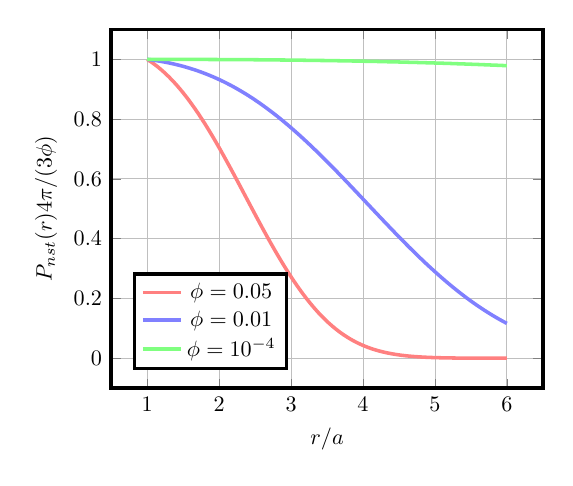
\begin{tikzpicture}[scale=0.8]
    \begin{axis}[
        xlabel={$r/a$},
        ylabel={$P_\text{nst}(r) 4\pi/ (3\phi) $},
        legend style={at={(0.05,0.05)}, anchor=south west},
        grid=major,
        domain=1:6,
        samples=100,
        ultra thick
    ]
    
    % Plot for phi = 0.05
    \addplot[color=red!50,ultra thick]
    { exp(-0.05 * (x^3 - 1))};
    \addlegendentry{$\phi = 0.05$}
    
    % Plot for phi = 0.01
    \addplot[color=blue!50,ultra thick]
    { exp(-0.01 * (x^3 - 1))};
    \addlegendentry{$\phi = 0.01$}
    
    % Plot for phi = 0.001
    \addplot[color=green!50,ultra thick]
    { exp(-0.0001 * (x^3 - 1))};
    \addlegendentry{$\phi = 10^{-4}$}
    
    \end{axis}
\end{tikzpicture}
\hfil
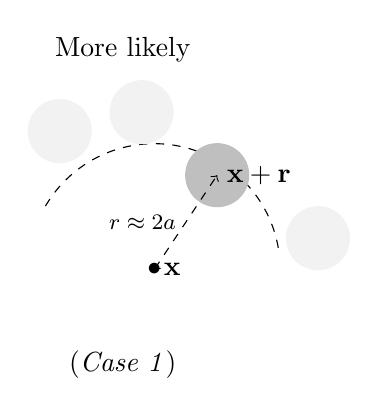
\begin{tikzpicture}[scale=0.8]
  \filldraw[ gray!10!white](+2.6,0.5)circle (0.5);
  \filldraw[ gray!10!white](-1.5,2.2)circle (0.5);
  \draw[dashed](10:2) arc (10:150:2);
  % \filldraw[ gray!50!white](0,0) circle (0.5);
  \filldraw[ gray!50!white](1,1.5)circle (0.5);
  \filldraw[ gray!10!white](-0.2,2.5)circle (0.5);
  \draw(0,0)node{$\bullet$}node[right]{$\textbf{x}$};
  \draw[dashed,<->](0,0)--(1,1.5)node[midway,left]{\footnotesize $r\approx 2 a$}node[right]{$\textbf{x}+\textbf{r}$};
  % \draw[dashed](-0.2,3.5);
  \node[ultra thick] (title) at (-0.5,3.5) {{More likely}};
  \node[ultra thick] (title) at (-0.5,-1.5) {(\textit{Case 1})};
\end{tikzpicture} 
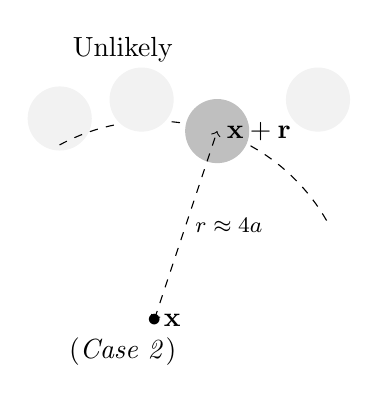
\begin{tikzpicture}[scale=0.8]
  \filldraw[ gray!10!white](+2.6,3.5)circle (0.5);
  \filldraw[ gray!10!white](-1.5,3.2)circle (0.5);
  \draw[dashed](30:3.16) arc (30:120:3.16);
  % \filldraw[ gray!50!white](0,0) circle (0.5);
  \filldraw[ gray!50!white](1,3)circle (0.5);
  \filldraw[ gray!10!white](-0.2,3.5)circle (0.5);
  \draw(0,0)node{$\bullet$}node[right]{$\textbf{x}$};
  \draw[dashed,<->](0,0)--(1,3)node[midway,right]{\footnotesize  $r\approx 4a$}node[right]{$\textbf{x}+\textbf{r}$};
  % \draw[dashed](-0.2,3.5);
  \node[ultra thick] (title) at (-0.5,4.3) {{Unlikely}};
  \node[ultra thick] (title) at (-0.5,-0.5) {(\textit{Case 2})};
\end{tikzpicture} 
\caption{(left) Plot of the normalized nearest neighbor distribution $P_\text{nst}$. 
(right) Sketches explaining the behavior of the nearest neighbor distribution $P_\text{nst}$: 
(\textit{Case 1}) A droplet located at $\textbf{x}+\textbf{r}$ relatively \underline{close} to a point occupied by the continuous phase at \textbf{x}; this situation is likely to happen. 
(\textit{Case 2}) A droplet located at $\textbf{x}+\textbf{r}$ relatively \underline{far} to a point occupied by the continuous phase at \textbf{x}; this situation very unlikely to happen.
Indeed, it implies that no particles are present within the sphere of radius $4a$ centered at $\textbf{x}$ since the nearest neighbor is located at a distance $4a$. 
}
\label{fig:P_nst_f}
\end{figure}



Before computing teh integration for Stokes flows we would like to apply this formulation to re-compute the \textit{Reynolds stress} of translating bubbles in potential flows. 
Therefore, we carry out the direct integration of \ref{eq:step_one} using \ref{eq:potential_sol} and obtain, 
\begin{equation}
    \avg{\chi_f \rho_f \textbf{u}_f'\textbf{u}_f'}
    = \Gamma_\text{inc}(-1,\phi)\phi^2 e^\phi \left\{
        \frac{1}{20}[\textbf{u}_{fp}\textbf{u}_{fp}+ \frac{1}{n_p}\pavg{\textbf{u}_\alpha\textbf{u}_\alpha}]
        + 
        \frac{3}{20} (\textbf{u}_{fp}\cdot \textbf{u}_{fp} + 2k_p)\bm\delta
    \right\},
    \label{eq:potential_nst}
\end{equation}
where $\Gamma_\text{inc}$ is the gamma incomplete function. 
According to \ref{eq:potential_nst} our results differ with \ref{eq:van_wingarden_sol} by a factor of $\Gamma_\text{inc}(-1,\phi)\phi^2 e^\phi$. 
Nevertheless, this inconsistency is easily solved noticing that $\Gamma_\text{inc}(-1,\phi)\phi^2 e^\phi \sim \phi + \mathcal{O}(\phi^2)$. 
Thus, we conclude that at the leading order, our methodology seem consistent with the classical conditional average methodology introduced by \citet{batchelor1972sedimentation}. 

Now that we have all the tools, let us carry out the direct integration of \ref{eq:step_one} for the wake of a spherical droplet in stokes flows. 
In dimensionless form \ref{eq:step_one} gives, 
\begin{equation}
    \avg{\chi_f  \textbf{u}_f'\textbf{u}_f'}^*
    = \phi    
    C_1
    \left\{
        \textbf{u}_{fp}\textbf{u}_{fp}+ \frac{1}{n_p}\pavg{\textbf{u}_\alpha\textbf{u}_\alpha}
        -\frac{1}{3} (\textbf{u}_{fp}\cdot \textbf{u}_{fp} + 2k_p)\bm\delta
    \right\},    
    + \phi C_2
    (\textbf{u}_{fp}\cdot \textbf{u}_{fp} + 2k_p)\bm\delta,
    \label{eq:final_closure}
\end{equation}
with,
\begin{align*}
    C_1(\phi,\lambda)
    = \frac{1}{20(1+l)^2}\left[
        \frac{9(2+3\lambda)^2}{4}\Gamma(1/3) \phi^{-1/3}
        - (27+82\lambda +62\lambda^2)
    \right],\\
    C_2(\phi,\lambda)
    = \frac{1}{6(1+l)^2}\left[
        \frac{(2+3\lambda)^2}{4}\Gamma(1/3) \phi^{-1/3}
        - (3+10\lambda +8\lambda^2)
    \right].
\end{align*}
We have decomposed the \textit{Reynolds stress} tensor into two contribution. 
The first one being, a traceless symmetric tensor, proportional to the functional $C_1$. 
The second contribution is the isotropic part of the \textit{Reynolds stress} tensor, which is proportional to $C_2$. 
This result deserves some comments. 

Firstly, we can note that, according to the value of $C_1$ and $C_2$, the \textit{pseudo turbulence} or \textit{Reynolds stress} induced by the translation of the droplets is higher for large values of $\lambda$. 
In other words the solid particle induce more wake than a bubble of the same size. 

Secondly, as witnessed by the presence of the term $\phi^{-1/3}$, in $C_1$ and $C_2$, we conclude that the solution obtained here is still consistent with the observation made in \ref{eq:real_error} or in \citet{caflisch1985variance}. 
Indeed, for an isolated droplet, i.e. when we take the limit, $\phi \to 0$, we obtain $\lim_{\phi \to 0} \avg{\chi_f \textbf{u}_f' \textbf{u}_f'} / \phi = \infty$. 
Consequently, in agreement with the previous statements, the normalized \textit{Reynolds stress} is infinite for an isolated droplet, however when considering small but finite value of $\phi$ the \textit{Reynolds stress} remains finite and is given by \ref{eq:final_closure}. 

Finally, as it is not the \textit{Reynolds stress} divided by $\phi$ that matter, but $\avg{\chi_f\textbf{u}_f'\textbf{u}_f'}$ it self, note that at the leading order in $\phi$ we obtain,  $\avg{\chi_f\textbf{u}_f'\textbf{u}_f'}\sim\phi^{2/3}$. 
Notably, this  trend in $\sim\phi^{2/3}$ is not new and agree with previous studies found in the literature, this will be examined in the next section. 

% of \citet{hill2001first} and \which computed the \textit{Reynolds stress} term in ordered and random array of solid spheres. 
